\section{Use Cases}
\subsection{General Use Case}

\begin{figure}[h!]
    \centering
    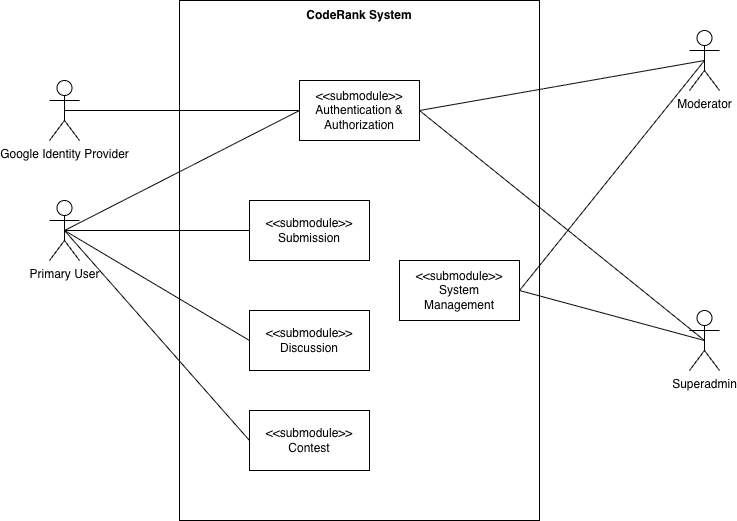
\includegraphics[width=1\textwidth]{Contents/Chapter 3/Usecase/Images/GeneralUsecase.png}
    \vspace{0.6cm}
    \caption{General Use Case}
\end{figure}


Our system contains 5 main submodules:
\begin{itemize}
    \item \textbf{Authentication \& Authorization}: Responsible for managing secure login and enforces Role-Based Access Control for 3 types of user.
    \item \textbf{Discussion}: Facilitates community interaction, allowing primary users to share solutions and ask questions related to problems. 
    \item \textbf{System Management}: The administrative interface used by Moderator and Superadmin to manage the problem creation, test cases, contests management and global user accounts.
Contest: Enables timed, high-stakes programming events with real-time ranking and automated leaderboards.
    \item \textbf{Submission}: This core module handles the presentation of the coding challenge and the automatic evaluation of the user's submitted solution.
\end{itemize}

\subsection{Use-case diagrams for each submodule}

\begin{figure}[h!]
    \centering
    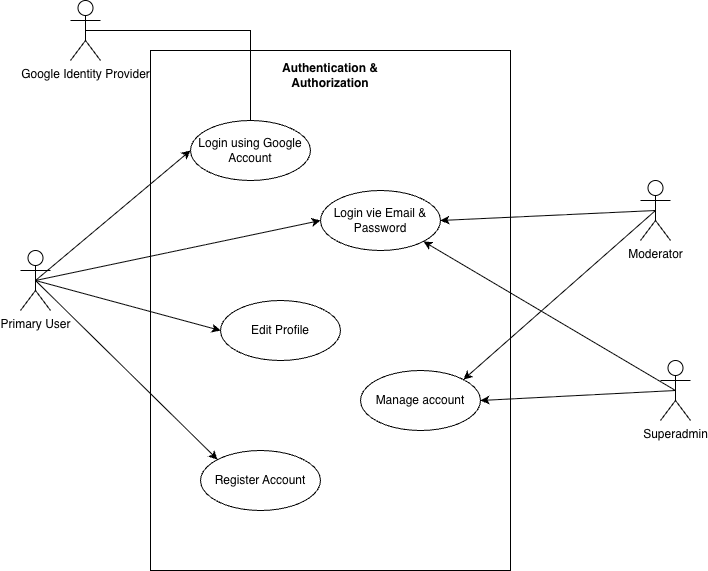
\includegraphics[width=1\textwidth]{Contents/Chapter 3/Usecase/Images/GeneralUsecase-Authentication.drawio.png}
    \vspace{0.6cm}
    \caption{Authentication \& Authorization Use Case}
\end{figure}
This submodule serves as the primary security gate for the entire system. Its core responsibility is to handle all user authentication (logging in) and authorization (managing access rights). This is crucial for protecting users' personal information, ensuring data privacy, and securing sensitive actions within the platform. By strictly controlling access, the module prevents unauthorized entry and maintains system integrity.
For user convenience, we offer diverse login methods:
\begin{itemize}
    \item Primary Users can log in quickly using their Google Account or use the traditional \textbf{Email \& Password} method.
    \item However, for privileged administrative roles—the Moderator and the Superadmin—access is strictly limited to the Login via \textbf{Email \& Password} method to enforce heightened security and traceability for system management functions.
\end{itemize}

All users retain standard account management capabilities, including registering a new account and changing their password.

\begin{figure}[h!]
    \centering
    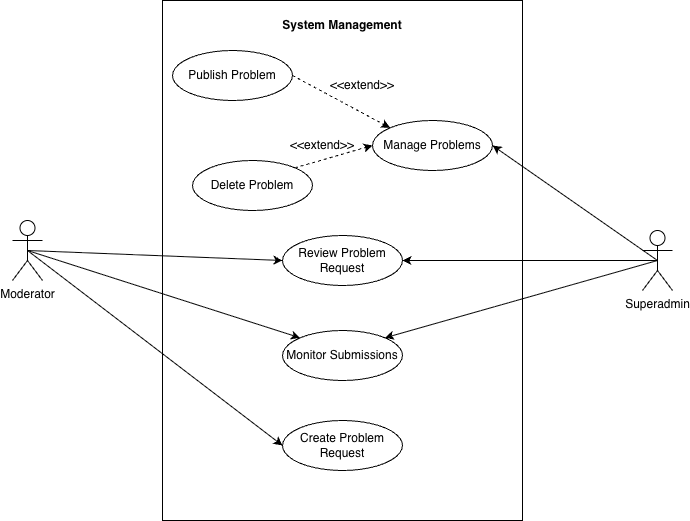
\includegraphics[width=1\textwidth]{Contents/Chapter 3/Usecase/Images/GeneralUsecase-SystemManagement.drawio.png}
    \vspace{0.6cm}
    \caption{System Management Use Case}
\end{figure}
The \textbf{System Management submodule} is the administrative dashboard used exclusively by the \textbf{Moderator} and \textbf{Superadmin} roles to control the content and operation of the platform.
\begin{itemize}
    \item \textbf{Problem Management}: Only Superadmin is enabled to manage problems directly (create, modify, delete) without reviewing steps
    \item \textbf{Content Workflow}: The Moderator initiates a Create Problem Request, and both the Moderator and Superadmin review problem requests before they go live.
    \item \textbf{Quality Control}: Both roles Monitor Submissions to track user activity, diagnose potential grading issues, and ensure fair play.
\end{itemize}
\clearpage

\begin{figure}[h!]
    \centering
    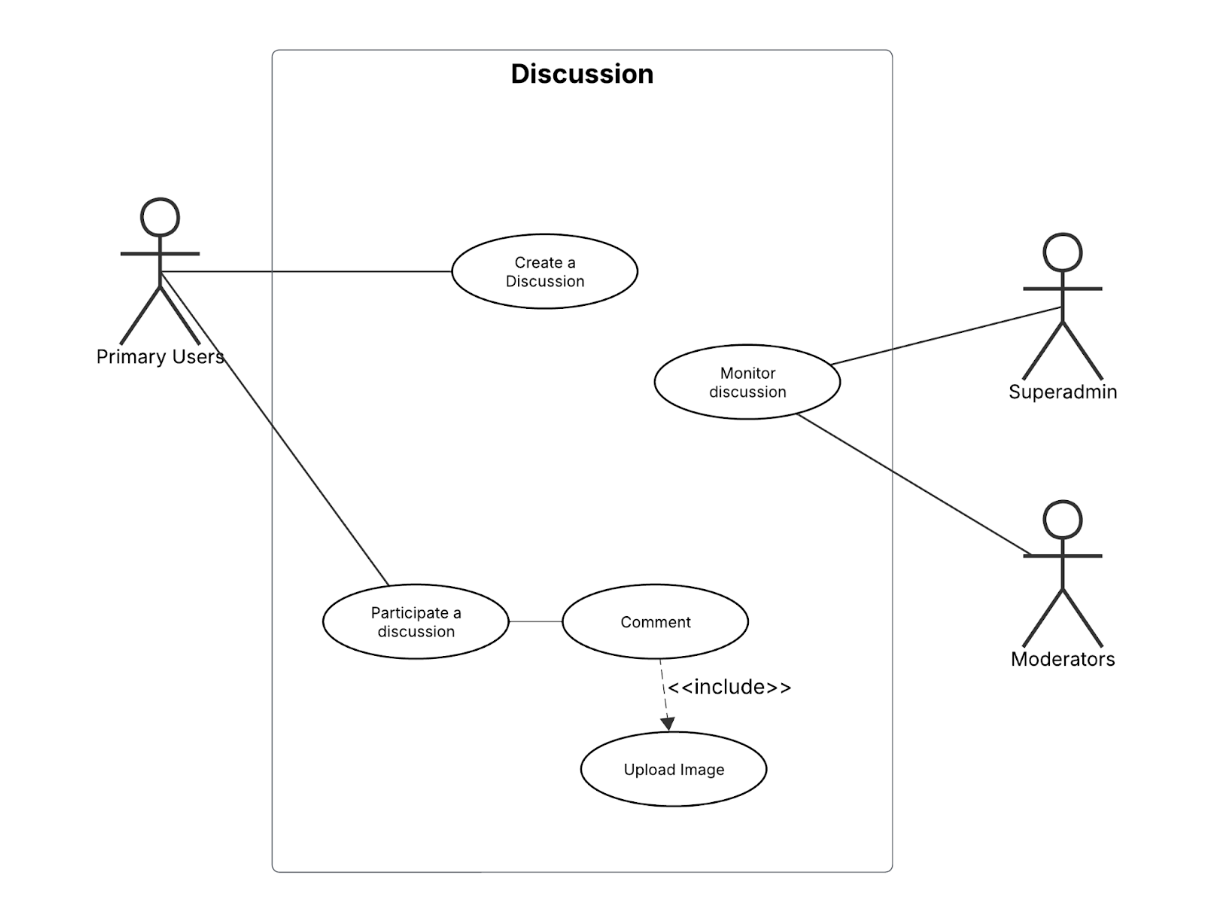
\includegraphics[width=1\textwidth]{Contents/Chapter 3/Usecase/Images/Discussion.png}
    \vspace{0.6cm}
    \caption{Discussion Use Case}
\end{figure}
The \textbf{Discussion submodule} helps make CodeRank a friendly and interactive community where users can learn from each other. With the Create Discussion feature, users can start new discussion threads about coding problems, programming ideas, or any tech-related topic. After a thread is created, others can join in by commenting on that thread. Comments can include rich content, such as images added, making explanations clearer and easier to follow.
To ensure that discussions remain constructive and aligned with community guidelines, the submodule integrates essential administrative controls. Both the Superadmin and Moderators utilize the Monitor Discussion function to oversee user activity, identify and address inappropriate content, and uphold the platform’s community standards. 

\clearpage

\begin{figure}[h!]
    \centering
    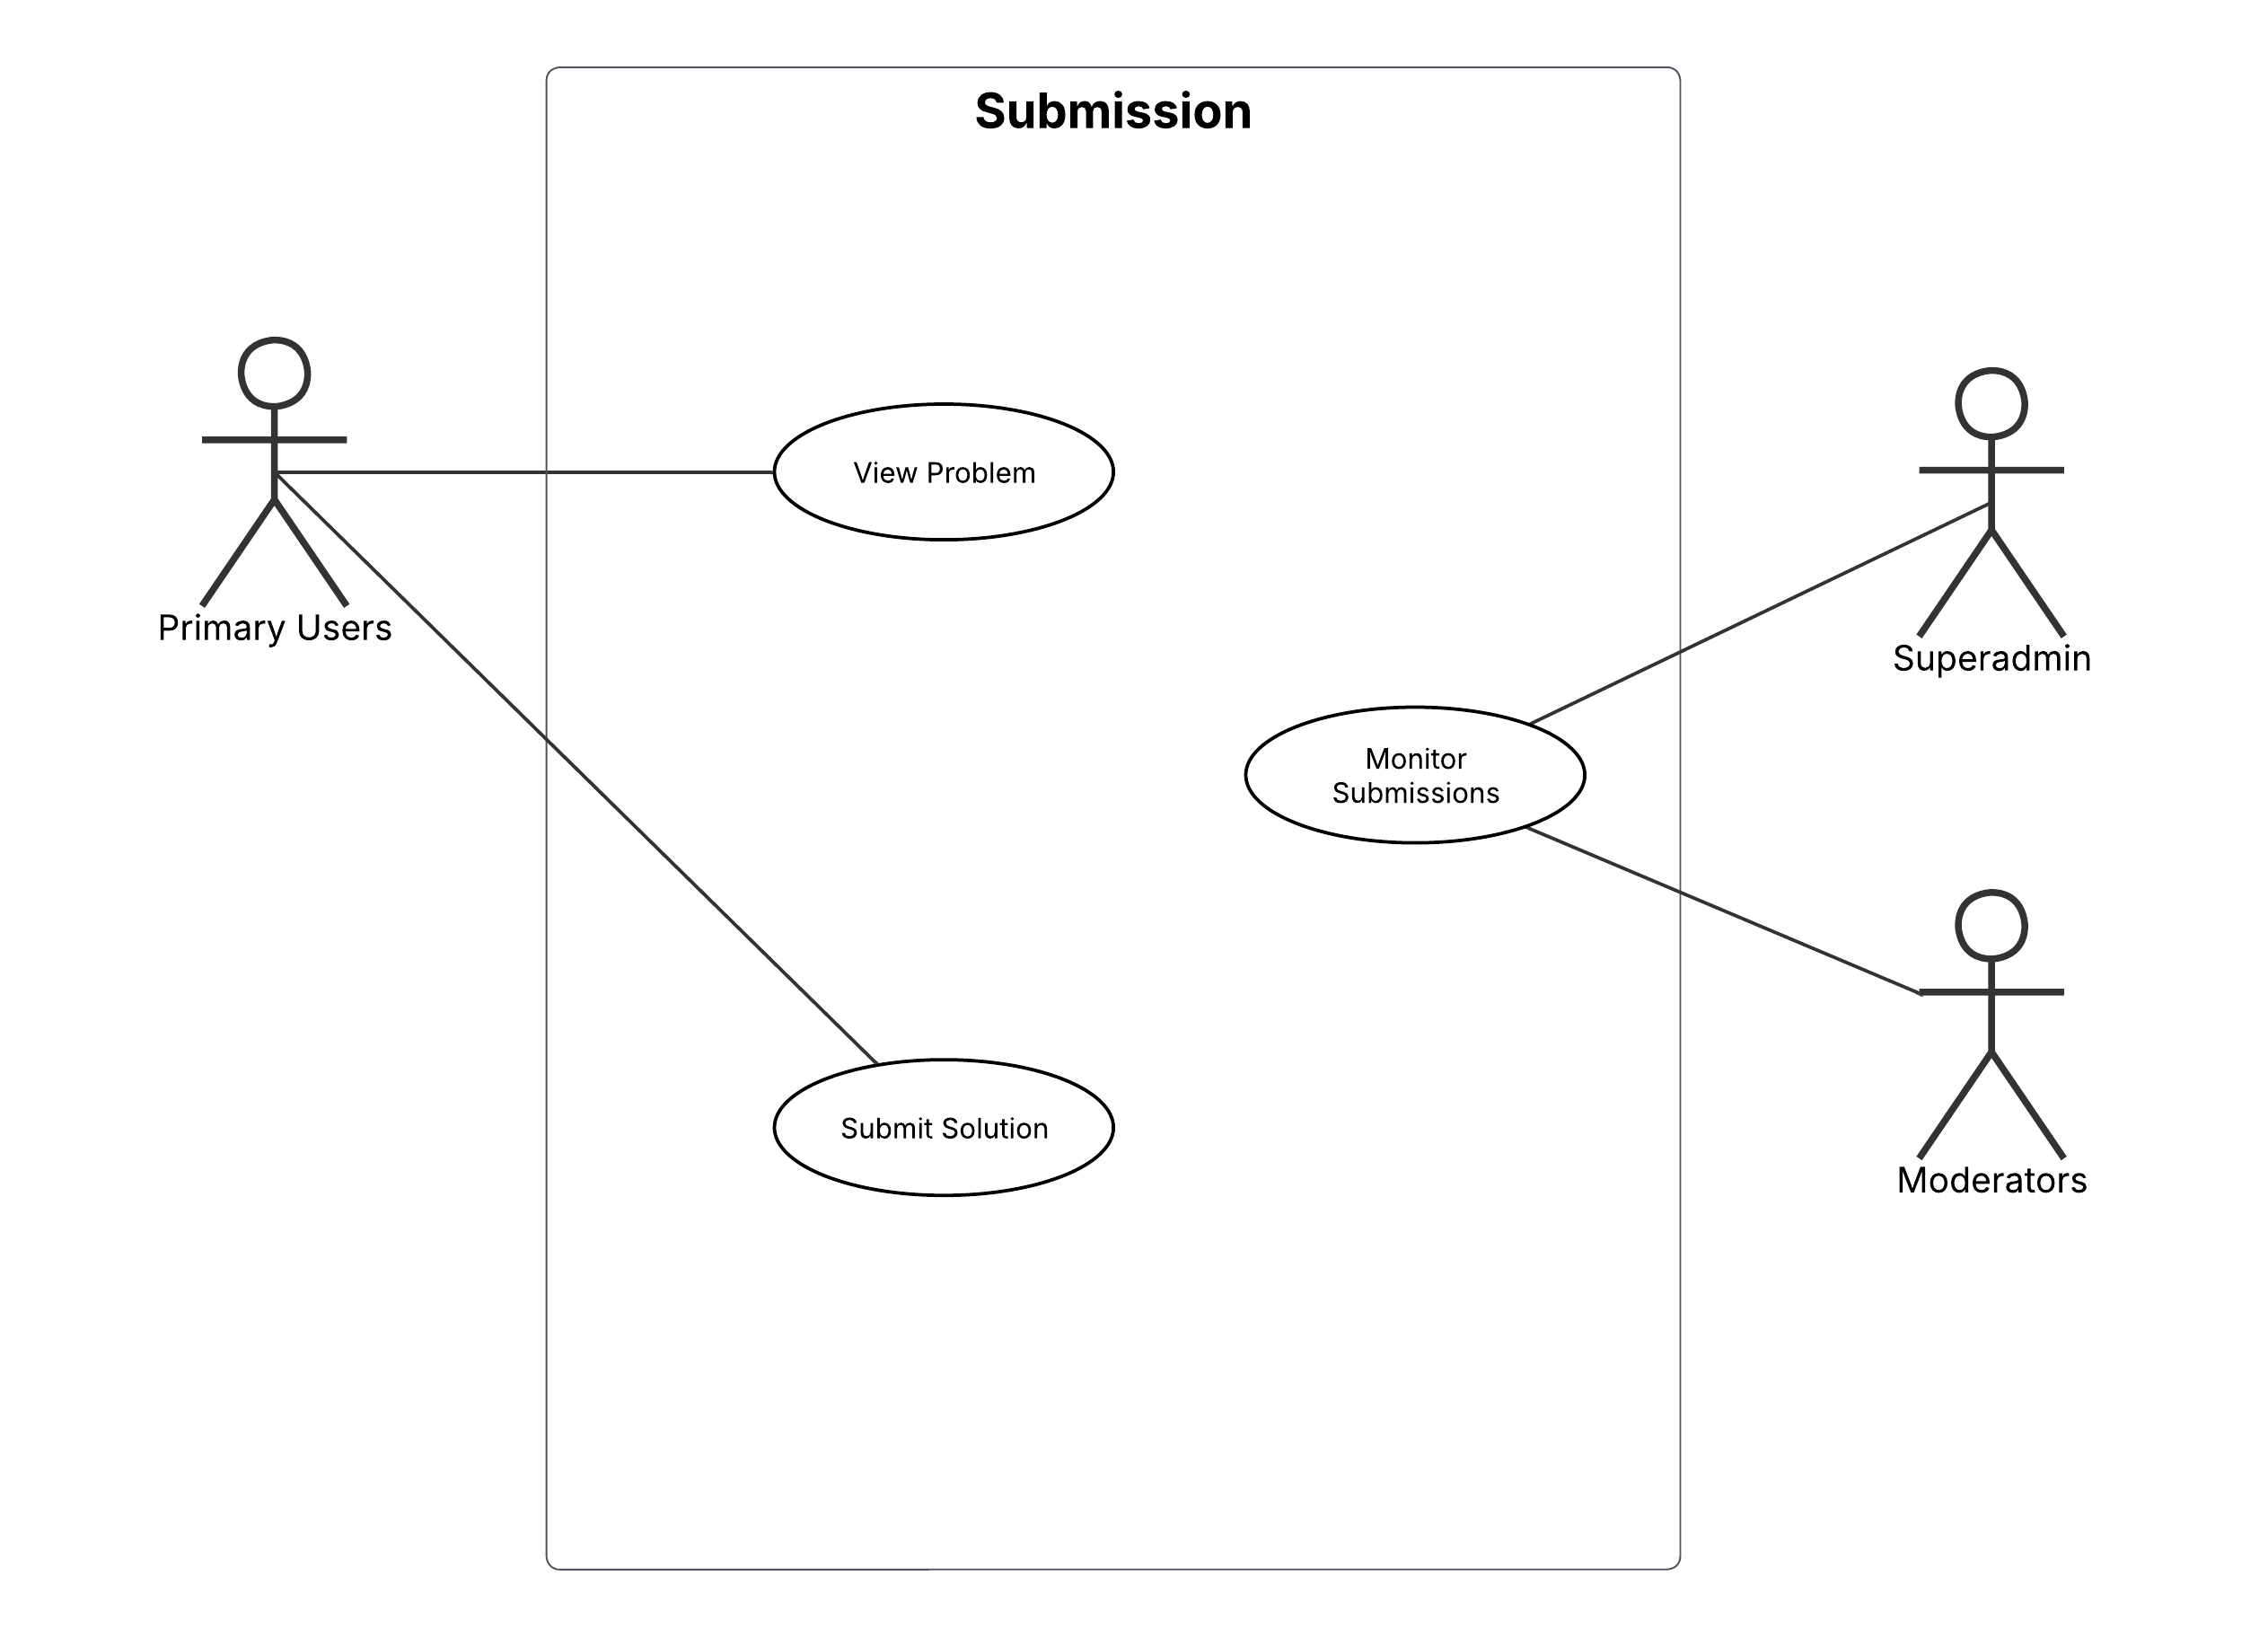
\includegraphics[width=1\textwidth]{Contents/Chapter 3/Usecase/Images/Submission.png}
    \vspace{0.6cm}
    \caption{Submission Use Case}
\end{figure}
The \textbf{Submission} submodule is the core execution engine and interaction point for all coding activities within the CodeRank system. Its primary function is to facilitate the practice and assessment workflow for the Primary User. Users begin by accessing the \textbf{View Problem} function, which presents the algorithmic challenge and requirements. The fundamental action in this module is the \textbf{Submit Solution} function, which securely receives the user's code, initiates the automatic grading process in a sandboxed environment, and returns the execution verdict. For oversight and quality assurance, both the Superadmin and Moderators are granted the ability to Monitor Submissions. This administrative function is vital for diagnosing issues with test cases, tracking potential cases of plagiarism, and ensuring the overall stability and fairness of the automated grading system.
\subsubsection{Use-case description tables}
% \begin{table}
% \caption{Use Case UC-1: Problems Management}
% \renewcommand{\arraystretch}{1.4}
% \begin{tabular}{|p{4cm}|p{11cm}|}
% \hline
% \textbf{ID and Name} & UC-1. Problems Management \\ \hline

% \textbf{Date Created} & 20th September, 2025 \\ \hline

% \textbf{Primary Actor} & Primary User, Superadmin, Moderator \\ \hline

% \textbf{Secondary Actor} & System (CodeRank Platform) \\ \hline

% \textbf{Description} &
% This use case describes how Moderators and Superadmins manage algorithmic problems on the platform. The process includes creating, editing, approving, and publishing problems. It also covers defining problem statements, input/output formats, constraints, sample test cases, and hidden test cases.
% \\ \hline

% \textbf{Trigger} &
% A Moderator or Superadmin decides to create, edit, approve, or publish a problem.
% \\ \hline

% \textbf{Preconditions} &
% \begin{itemize}
% \item The user is logged in as a Moderator or Superadmin.
% \item The problem management interface is accessible.
% \end{itemize}
% \\ \hline

% \textbf{Postconditions} &
% \begin{itemize}
% \item A new problem is created and saved as draft.
% \item A draft problem is updated or submitted for approval.
% \item A published problem may be updated after Superadmin approval.
% \item A problem is published once the approval rule is satisfied.
% \end{itemize}
% \\ \hline

% \textbf{Normal Flow} &
% \begin{enumerate}
% \item Moderator/Superadmin accesses the problem management interface.
% \item Moderator creates a new problem (saved as draft).
% \item Moderator edits draft problem (auto-saved).
% \item Moderator or Superadmin submits the problem for approval.
% \item Moderator approves problem → System checks publishing rule.
% \item If approvals >= 3 (Moderators) or 1 (Superadmin), system auto-publishes.
% \item Superadmin can directly approve and publish a problem.
% \end{enumerate}
% \\ \hline

% \textbf{Alternative Flow} &

% \textbf{AF–1:} Moderator edits a published problem → System saves changes as pending\_edit → Requires Superadmin approval. 

% \textbf{AF–2:} If approval threshold is not met, the problem stays pending until more approvals are collected.
% \\ \hline

% \textbf{Exceptions} &
% \textbf{E–1:} Superadmin rejects a pending edit → System notifies Moderator.
% \\ \hline
% \end{tabular}
% \end{table}


% \begin{table}
% \caption{Use Case UC-2: Contest Management}
% \renewcommand{\arraystretch}{1.3}
% \begin{tabular}{|p{4cm}|p{11cm}|}
% \hline
% \textbf{ID and Name} & UC-2. Contest Management \\ \hline

% \textbf{Date Created} & 20th September, 2025 \\ \hline

% \textbf{Primary Actor} & Primary User, Superadmin, Moderator \\ \hline

% \textbf{Secondary Actor} & System (CodeRank Platform) \\ \hline

% \textbf{Description} &
% This use case describes how users create and submit contests, allow administrators to review and approve them, and make contests available for participation once published.
% \\ \hline

% \textbf{Trigger} &
% A Primary User submits a new contest request.
% \\ \hline

% \textbf{Preconditions} &
% \begin{itemize}[nosep, leftmargin=*]
% \item The user is authenticated.
% \item Contest details (title, description, rules, problems) are provided.
% \item The contest submission form is valid.
% \end{itemize}
% \\ \hline

% \textbf{Postconditions} &
% \begin{itemize}[nosep, leftmargin=*]
% \item Contest status is updated (pending, approved, or published).
% \item Notifications are sent to users and admins.
% \item Users can participate in contests once published.
% \end{itemize}
% \\ \hline

% \textbf{Normal Flow} &
% \begin{enumerate}[nosep, leftmargin=*]
% \item Primary User submits a contest request.
% \item The System saves the contest as \textit{Pending Review}.
% \item Moderators review and approve the contest.
% \item If at least 3 moderator approvals are received, the contest qualifies for publishing.
% \item Alternatively, a Superadmin may approve and publish with a single approval.
% \item The System updates the contest status to \textbf{Published}.
% \item Notifications are sent to the contest creator and relevant moderators.
% \item Primary Users may now participate in the contest.
% \end{enumerate}
% \\ \hline

% \textbf{Alternative Flow} &
% \begin{itemize}[nosep, leftmargin=*]
% \item \textbf{AF-1: Insufficient Approvals}: If fewer than 3 moderator approvals are received, the contest remains in \textit{Pending Review}.
% \item \textbf{AF-2: Superadmin Override}: A Superadmin may publish directly, bypassing moderator approvals.
% \item \textbf{AF-3: Invalid Submission}: If contest data is incomplete or invalid, the submission is rejected with an error message.
% \end{itemize}
% \\ \hline

% \textbf{Exceptions} &
% \begin{itemize}[nosep, leftmargin=*]
% \item \textbf{E-1}: Database error when saving or updating the contest request.
% \item \textbf{E-2}: Approval action references a contest that does not exist.
% \item \textbf{E-3}: Notification delivery fails (system logs error, but contest status remains updated).
% \end{itemize}
% \\ \hline

% \end{tabular}
% \end{table}

% \begin{table}

% \renewcommand{\arraystretch}{1.3}
% \begin{tabular}{|p{4cm}|p{11cm}|}
% \caption{Use Case UC-3: Create a Discussion}
% \hline
% \textbf{ID and Name} & UC-3. Create a Discussion \\ \hline

% \textbf{Date Created} & 20th September, 2025 \\ \hline

% \textbf{Primary Actor} & Primary User \\ \hline

% \textbf{Secondary Actor} & System (CodeRank Platform) \\ \hline

% \textbf{Description} &
% This use case describes how a \textbf{Primary User} initiates a new discussion thread, typically linked to a specific problem ID or a general topic, setting the initial content and title.
% \\ \hline

% \textbf{Trigger} &
% The Primary User navigates to a problem page or the main forum and selects the \textit{"New Discussion"} option.
% \\ \hline

% \textbf{Preconditions} &
% \begin{itemize}[nosep, leftmargin=*]
% \item The user is authenticated.
% \item The discussion creation interface is accessible.
% \end{itemize}
% \\ \hline

% \textbf{Postconditions} &
% \begin{itemize}[nosep, leftmargin=*]
% \item A new discussion thread is created with the status \textit{"Active."}
% \item The discussion is visible to other Primary Users.
% \end{itemize}
% \\ \hline

% \textbf{Normal Flow} &
% \begin{enumerate}[nosep, leftmargin=*]
% \item Primary User accesses the problem/forum page and initiates creation.
% \item The user enters the discussion title and body content.
% \item The user submits the discussion.
% \item The system saves the new thread, assigns a unique ID, and displays it.
% \end{enumerate}
% \\ \hline

% \textbf{Alternative Flow} &
% \begin{itemize}[nosep, leftmargin=*]
% \item \textbf{AF-1: Content Validation Error}: If the title or body content is empty, the System displays an error message and requires the User to correct the input before submission.
% \end{itemize}
% \\ \hline

% \textbf{Exceptions} &
% \begin{itemize}[nosep, leftmargin=*]
% \item \textbf{E-1: Submission Failure}: If the database connection fails, the System displays a technical error and saves the content as a temporary draft (if possible).
% \end{itemize}
% \\ \hline

% \end{tabular}
% \end{table}

% \newpage

% \begin{table}[h!]
% \renewcommand{\arraystretch}{1.3}
% \begin{tabular}{|p{4cm}|p{11cm}|}
% \caption{Use Case UC-4: Submit a Solution}
% \hline
% \textbf{ID and Name} & UC-4. Submit a Solution \\ \hline

% \textbf{Date Created} & 20th September, 2025 \\ \hline

% \textbf{Primary Actor} & Primary User \\ \hline

% \textbf{Secondary Actor} & System (CodeRank Platform), Worker Service \\ \hline

% \textbf{Description} &
% This use case describes the primary mechanism for a \textbf{Primary User} to select a programming language, submit their solution code for a problem they are currently viewing, and receive an automated verdict on its correctness and efficiency.
% \\ \hline

% \textbf{Trigger} &
% The Primary User clicks the \textit{"Submit"} button on a coding problem interface after entering or selecting their solution code.
% \\ \hline

% \textbf{Preconditions} &
% \begin{itemize}[nosep, leftmargin=*]
% \item The user is authenticated.
% \item The user is currently viewing an active problem.
% \item The user has selected a supported programming language.
% \item The code is syntactically valid (pre-checked client-side).
% \end{itemize}
% \\ \hline

% \textbf{Postconditions} &
% \begin{itemize}[nosep, leftmargin=*]
% \item The submitted code is sent to the System.
% \item The Submission History is updated with the result (e.g., Accepted, Wrong Answer).
% \item The user's score and statistics are updated based on the verdict.
% \end{itemize}
% \\ \hline

% \textbf{Normal Flow} &
% \begin{enumerate}[nosep, leftmargin=*]
% \item Primary User is on the problem page and selects their preferred language.
% \item The user enters or pastes the solution code into the editor.
% \item The user clicks \textit{"Submit."}
% \item The system validates the submission (e.g., code length, language availability).
% \item The system sends the code and the problem's hidden test cases to the Worker Service.
% \item \textbf{Worker Service} securely executes the code and determines the verdict (e.g., Accepted, Time Limit Exceeded, Runtime Error).
% \item The system displays the final verdict and execution statistics to the Primary User.
% \end{enumerate}
% \\ \hline

% \textbf{Alternative Flow} &
% \begin{itemize}[nosep, leftmargin=*]
% \item \textbf{AF-1: Attempted Language Not Supported}:  
% If the user attempts to submit code in a language that is not currently enabled for the problem, the System displays an error and requires the user to change their language selection.
% \end{itemize}
% \\ \hline

% \textbf{Exceptions} &
% \begin{itemize}[nosep, leftmargin=*]
% \item \textbf{E-1: Submission Failure}:  
% If the sandbox environment or the external grading service fails during execution, the System logs the error and returns a \textit{"System Error"} verdict to the user, advising them to try again later.
% \end{itemize}
% \\ \hline

% \end{tabular}
% \end{table}

